\documentclass{article}

\usepackage{graphicx}
\usepackage[margin=10pt,font=small,labelfont=bf]{caption}
\usepackage{subcaption}

\graphicspath{ {./../images} }

\begin{document}
\section*{Screenshots}

\begin{figure}[htp]
    \centering
    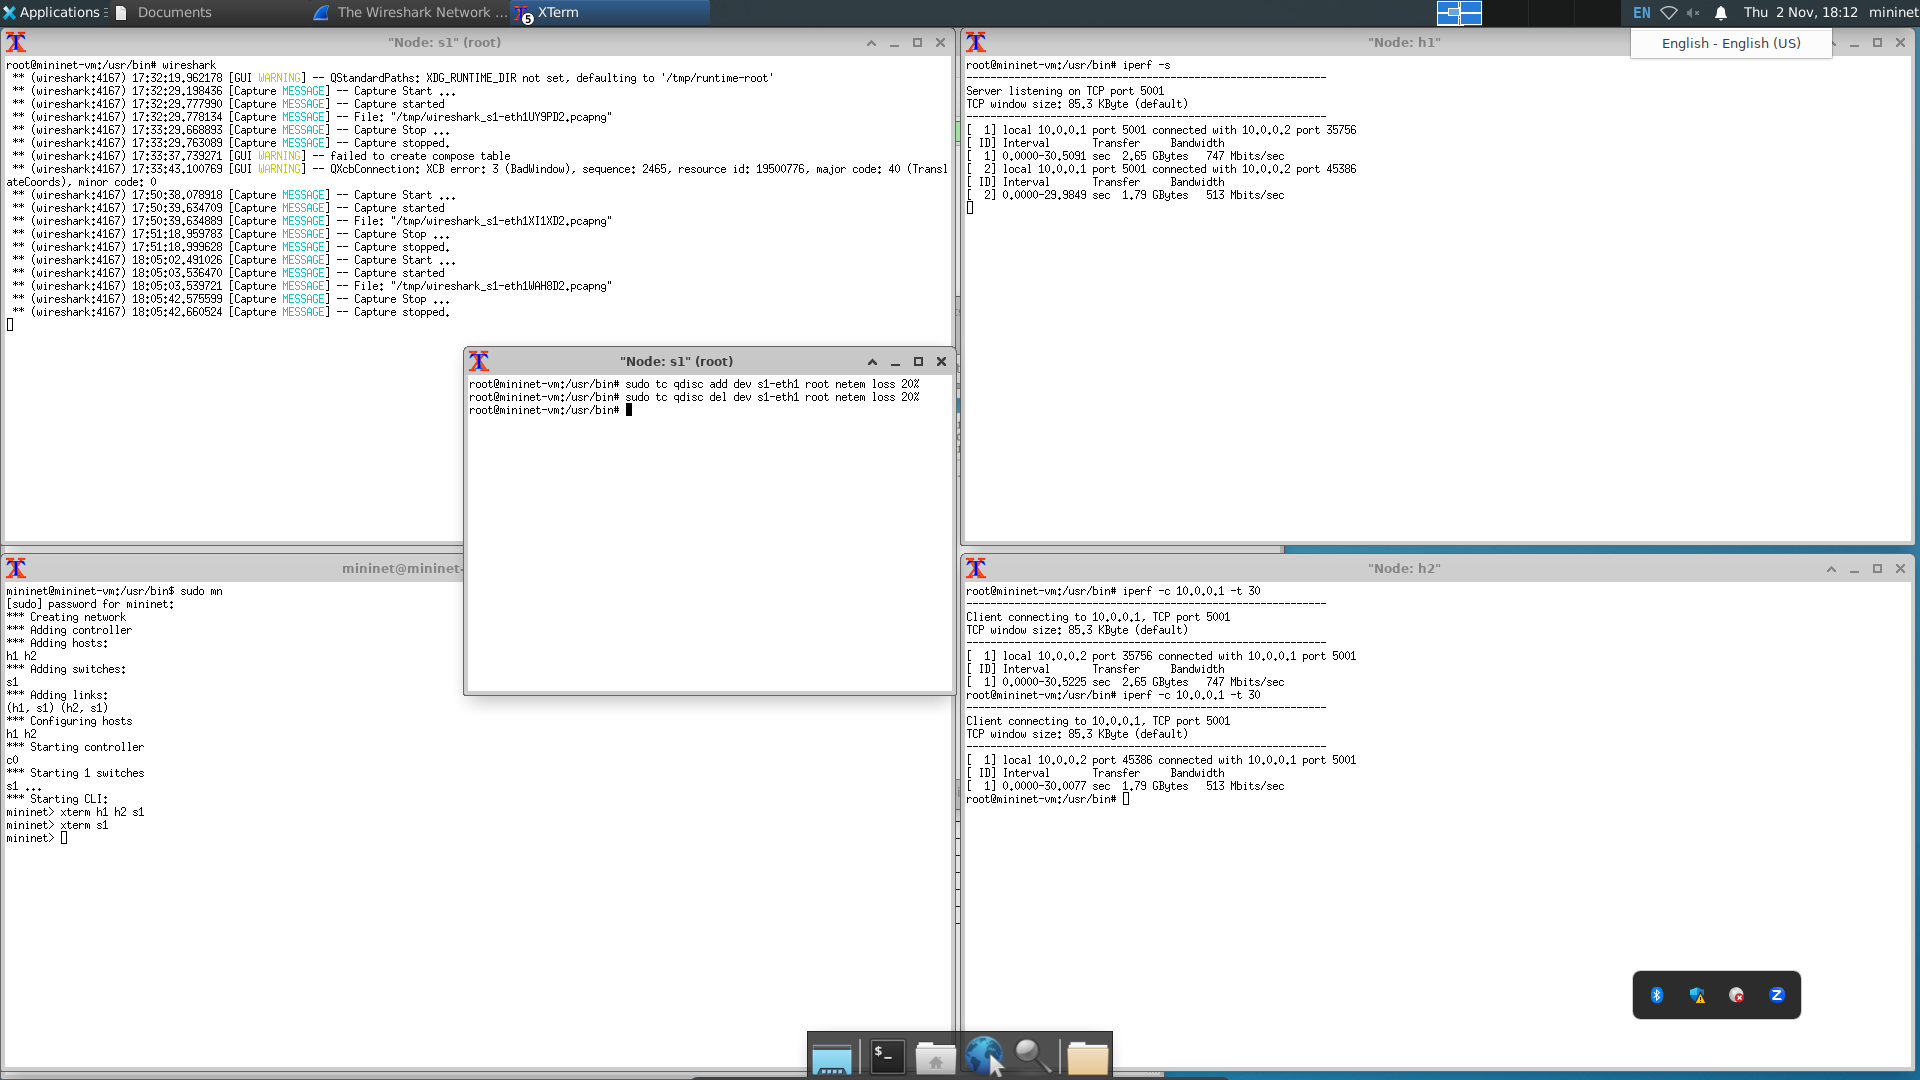
\includegraphics[width=\textwidth]{screenshot}
    \caption{Terminals}
\end{figure}

\begin{figure}[htp]
    \centering
    \begin{subfigure}{.5\textwidth}
        \centering
        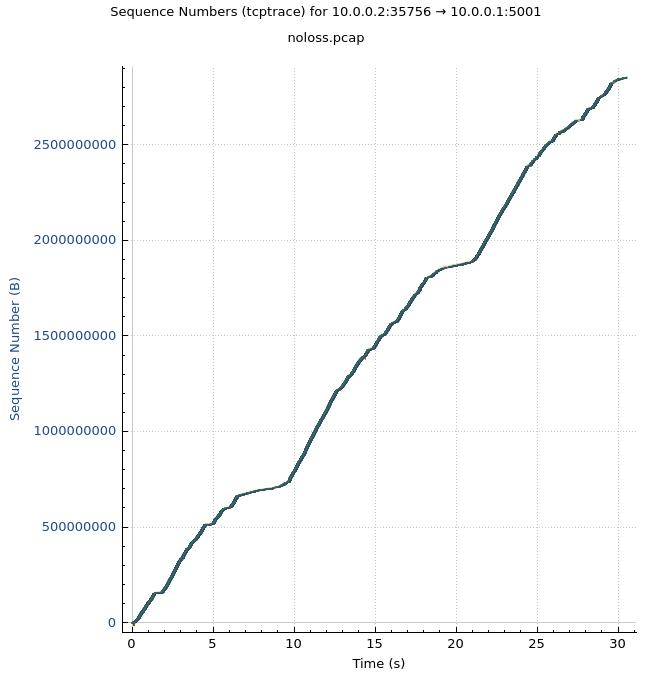
\includegraphics[width=\linewidth]{nolosstcptrace}
        \caption{Tcptrace}
    \end{subfigure}%
    \begin{subfigure}{.5\textwidth}
        \centering
        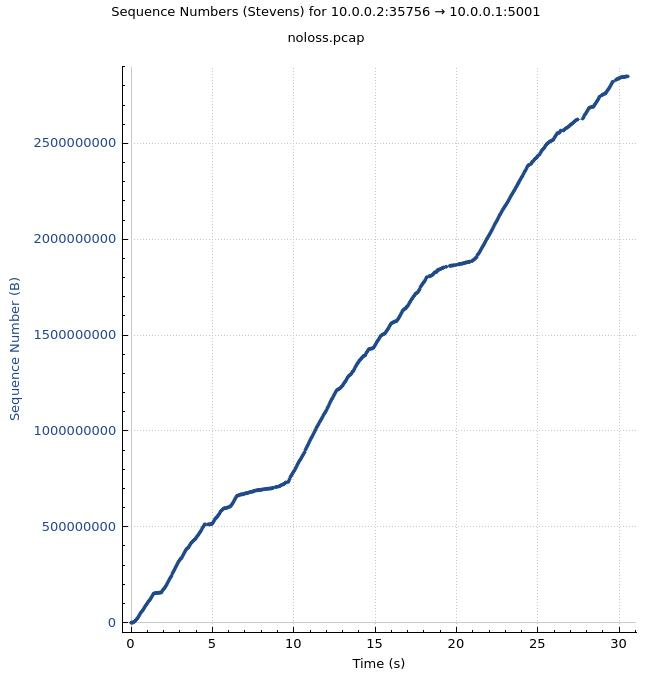
\includegraphics[width=\linewidth]{nolossstevens}
        \caption{Stevens}
    \end{subfigure}
    \caption{No Loss}
\end{figure}


\begin{figure}[htp]
    \centering
    \begin{subfigure}{.5\textwidth}
        \centering
        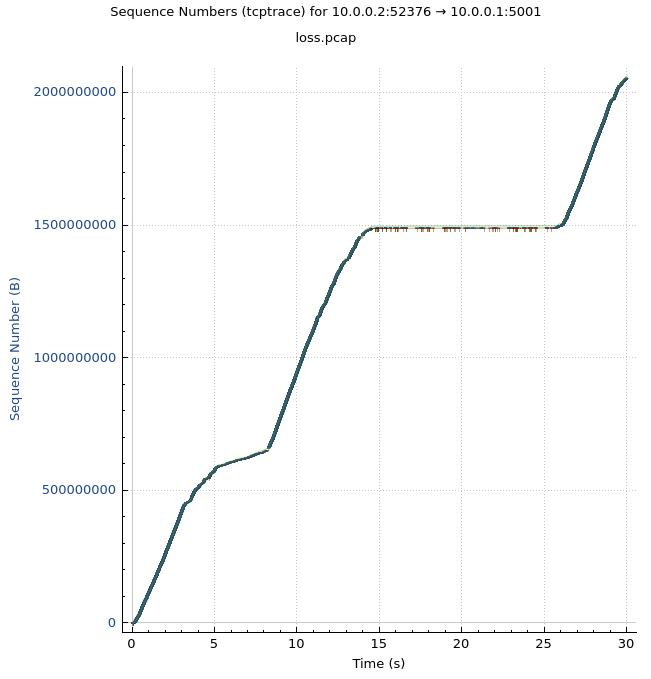
\includegraphics[width=\linewidth]{losstcptrace}
        \caption{Tcptrace}
    \end{subfigure}%
    \begin{subfigure}{.5\textwidth}
        \centering
        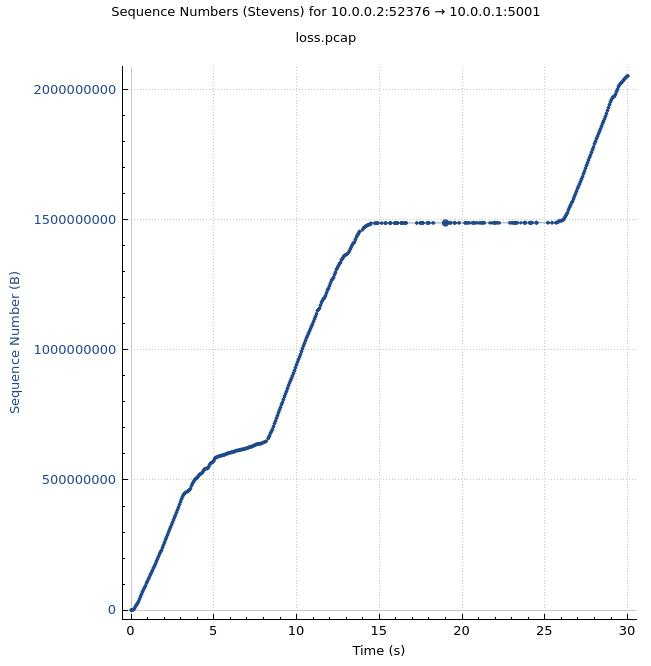
\includegraphics[width=\linewidth]{lossstevens}
        \caption{Stevens}
    \end{subfigure}
    \caption{Loss}
\end{figure}

\clearpage
\section*{Questions}
\subsection*{No Loss}
\noindent
On the time-sequence graph (tcp trace) with no loss, identify the regions of slow start and congestion avoidance.

The slow start is in the begging of the graph. (hard to see)

The rest of the time congestion avoidance.

\subsection*{Loss}
\noindent
On the time-sequence graph in the loss case, identify the region where the loss started.

From around 15th to 25th second.

\noindent
Identify areas where slow start and congestion avoidance was used.

The slow start is in the begging of the graph. (hard to see)

The rest of the time congestion avoidance.

\noindent
Did you see any occurrence of fast recovery? If so, did it affect the congestion window?

Yes during the packet loss period, the congestion window decreased. After the loss is over the fast recovery happens, with the window increasing rapidly till it saturates the bandwith.

\noindent
Is there a difference in throughput for the case with loss and no loss?

Yes without loss more data was transfered succesfuly.


\end{document}